% Results plan for the COMP438/538 project. Working document, not a graded deliverable.
% The target is Halil's. Dagger items and the draft fail conditions are Claude's, not Halil's.
% Yellow cells stay empty until measured. Build: pdflatex results_plan.tex (run twice).
\documentclass[10pt]{article}
\usepackage[a4paper,landscape,margin=1.5cm]{geometry}
\usepackage[T1]{fontenc}
\usepackage{lmodern}
\usepackage{microtype}
\usepackage{amsmath}
\usepackage{array,booktabs,tabularx}
\usepackage[table]{xcolor}
\usepackage{float}
\usepackage[font=small,skip=3pt,justification=raggedright,singlelinecheck=false]{caption}
\usepackage{tikz}
\usepackage{titlesec}
\usepackage[hidelinks]{hyperref}

\titlespacing*{\section}{0pt}{10pt}{4pt}
\titlespacing*{\subsection}{0pt}{8pt}{3pt}
\setlength{\parindent}{0pt}
\setlength{\parskip}{4pt}
\renewcommand{\arraystretch}{1.2}
\setlength{\tabcolsep}{4pt}

\newcolumntype{L}{>{\raggedright\arraybackslash}X}
\newcolumntype{Y}{>{\centering\arraybackslash}X}
\newcolumntype{P}[1]{>{\raggedright\arraybackslash}p{#1}}
\newcommand{\E}{\cellcolor{yellow!40}}
\newcommand{\my}{\textsuperscript{\textcolor{blue!70!black}{\dag}}}
\newcommand{\pub}{\rowcolor{gray!16}}

\begin{document}

\begin{center}
  {\Large Results plan: System One Control of LLM Agent Harnesses with Verifiable Rewards}\\[3pt]
  COMP438/538 project, Halil Kanpak. Working plan of 3 November 2026, not graded. Nothing here has been run.
\end{center}

\section{The target}

Make Gemma-4-E4B reach the success of Qwen3.8-27B on ALFWorld by putting a trained System One model (Sys1) in front of it. The target is yours. Every other table in this plan supports the middle row below.

\begin{table}[H]
\footnotesize
\caption{The project in three rows. Published numbers are from the Bonn benchmark, 134 ALFWorld games, with thinking off and no text generated.}
\label{t:target}
\begin{tabularx}{\linewidth}{@{}P{7.5cm} P{3.4cm} Y Y@{}}
\toprule
Who plays the game & Model size & Published success (\%) & Our success (\%) \\
\midrule
Gemma alone & 8.0B (4.5B effective) & 6.7 [3.0, 11.2] & \E \\
Gemma + trained Sys1 (the result we want) & 8.0B + 4.7B & None & \E \\
Qwen 27B alone & 27.8B & 54.5 [46.3, 62.7] & \E \\
\bottomrule
\end{tabularx}
\end{table}

Reading key: \colorbox{yellow!40}{yellow cell} stays empty until measured. \colorbox{gray!16}{gray row} is a published number from someone else's setup. A dagger\my{} marks a choice Claude proposed, which you can veto. Every choice, who made it, every hyperparameter, the open decisions D1 to D6 and the draft fail conditions are in \texttt{choices.pdf} beside this file.

\section{Words used in this plan}

\begin{table}[H]
\scriptsize
\renewcommand{\arraystretch}{1.08}
\caption{Glossary. These words mean only this throughout the plan.}
\label{t:words}
\begin{tabularx}{\linewidth}{@{}P{2.5cm} L P{2.5cm} L@{}}
\toprule
\multicolumn{2}{@{}l}{The players} & \multicolumn{2}{l@{}}{Training} \\
\midrule
Sys1 & Picks one option from a list and gives a probability for each option. It writes no text, so it is fast. Same kind of model as Jev. Ours is Kev-4B, trained further & Teacher & Whoever supplies the right command during training: ALFWorld's built-in expert program, or a strong LLM (decision D1) \\
Gemma, Qwen 27B & The two LLMs: Gemma-4-E4B (small) and Qwen3.8-27B (large). An LLM writes text, so it is slow & Arm & One way of training Sys1. There are five, A0 to A4 (Table~\ref{t:arms}) \\
Harness & The loop around the models. At each step it decides who acts, runs the command and records the output & Classification & Train Sys1 to copy the teacher's pick, with no RL \\
Gemma + Sys1 & The harness with Sys1 in control, handing the steps it cannot take to Gemma & Teacher forcing & During training the teacher's command runs, whatever Sys1 picked \\
\cmidrule(r){1-2}
\multicolumn{2}{@{}l}{One game} & Model in control & During training Sys1's own command runs, mistakes included \\
\cmidrule(r){1-2}
ALFWorld & A text game of household tasks, such as ``put a clean apple in the fridge'' & Step match & How often Sys1's pick equals the teacher's pick \\
Episode, step & An episode is one game of at most 50 steps. A step is one command & Confidence & The probability Sys1 gives its own pick \\
Success & The game's own checker says the task is done. This is the verifiable part of the return & Calibrated & When Sys1 says 80\%, it is right about 80\% of the time. ECE measures the gap, and lower is better \\
Admissible commands & The commands the game allows at this step, 15 to 44 in ALFWorld & Exposure gap & Step match on situations the teacher reached, minus step match on situations Sys1 reached by itself \\
\cmidrule(l){3-4}
Menu & The short list Sys1 chooses from: the $k$ admissible commands the teacher used most in similar situations, counted on training games. $k$ is a hyperparameter tuned on dev, starting at 10 & \multicolumn{2}{l@{}}{Reading the results} \\
\cmidrule(l){3-4}
Fallback & Sys1's menu option that means ``LLM, you take this step'' & Dev, test & Dev is 140 games for tuning choices. Test is 134 games, played once at the end \\
Control state & Three numbers Sys1 sees: who controls now, fallbacks in a row, LLM rounds left & 95\% interval & The plausible range of a number, given the games played. Written [low, high] \\
Repeat rate & Share of steps that repeat an earlier command. High means a mistake loop & Ablation & Switch one part off, run again and see whether success drops \\
Handover & One step given to Qwen 27B, one call. Q5 counts these and lasts one step, unlike the hand-over rules & Bonn, ReDAct & The two main comparison papers. Bonn tests Jev, Gemma and Qwen 27B on ALFWorld. In ReDAct a small LLM hands steps to a large one when unsure, with no training \\
\bottomrule
\end{tabularx}
\end{table}

\section{The story, one question per table}

\begin{table}[H]
\footnotesize
\caption{Each question is asked because the one before it had an answer. G and Q1 check the ground, Q2 and Q3 are the RL part, Q4 is the target, and Q5 to Q7 say what the result costs, protects and depends on.}
\label{t:story}
\begin{tabularx}{\linewidth}{@{}c L P{7.6cm} c c@{}}
\toprule
\# & Question & What we measure & Table & Page \\
\midrule
G & Do we get the published numbers for Gemma and Qwen 27B in our own setup? & Success on Bonn's 134 games & \ref{t:gate} & \pageref{t:gate} \\
Q1 & How often is the right next command on the short menu? If often, Sys1 can take those steps and Gemma is left with the hard ones & Share of teacher commands on the menu, and each LLM alone on dev & \ref{t:q1} & \pageref{t:q1} \\
Q2 & After training, how often does Sys1 pick the teacher's command, and is its confidence honest? & Step match and calibration of each arm & \ref{t:q2} & \pageref{t:q2} \\
Q3 & Does RL train Sys1 better than plain copying, and should the teacher's or Sys1's commands run during training? & Success of Sys1 alone for each arm, and the exposure gap & \ref{t:q3} & \pageref{t:q3} \\
Q4 & Does Gemma + Sys1 reach Qwen 27B? (the target) & Success and cost on the test games & \ref{t:main} & \pageref{t:main} \\
Q5 & If a few steps per game may go to Qwen 27B, how much does success rise, and who should choose those steps: chance, Gemma's own uncertainty, or Sys1? & Success at 1, 2, 5 and 10 handovers per game & \ref{t:q5} & \pageref{t:q5} \\
Q6 & Can Sys1 stop prompt injections by checking each tool call, and does it help that Sys1 never reads the tool output where the attack sits? & Attack success and task success on AgentDojo & \ref{t:q6} & \pageref{t:q6} \\
Q7 & Which parts of our design actually help? & Ablations of the menu, control state, reward and hand-over rules & \ref{t:abl} & \pageref{t:abl} \\
\bottomrule
\end{tabularx}
\end{table}

\section{What we run}

\begin{table}[H]
\footnotesize
\caption{Tasks. The harness reads the admissible actions and the success check from the environment on every task. ALFWorld is primary\my{} because Bonn and ReDAct both report on it, its checker is free, and it needs no simulated user. Outside the core: ScienceWorld as an extension (SwiftSage), CyberGym's 10-task subset as counts if a Docker host exists, and BFCL v4 with ToolRet for the reduced project (Clef card, CLM post).}
\label{t:tasks}
\begin{tabularx}{\linewidth}{@{}P{2cm} P{4.6cm} P{3.6cm} P{3.2cm} L P{3cm}@{}}
\toprule
Role & Task and setup & Train / dev / test & Admissible actions & Teacher available for free & Who else reports on it \\
\midrule
Primary\my & ALFWorld text (\texttt{AlfredTWEnv}), 6 task types, 50-step cap & 3,553 games / 140 \texttt{valid\_seen} / 134 \texttt{valid\_unseen} & Listed by the game, 15 to 44 per step (Bonn) & Built-in expert (\texttt{expert\_plan}). Its ties use a global random draw, so seed per episode as Bonn does & Bonn on these exact games. ReDAct on 400 episodes \\
Second, cheap RL\my & MiniGrid-DoorKey-8x8-v0, full view as text, 50-step cap & New seeds\my{} / seed 993 / 200 episodes from seed 42 & The environment's fixed actions, so menu length does not apply & Shortest-path solver that we write\my & ReDAct on this setup. When2Ask on a close variant \\
Guardrail, and the literal tool calling & AgentDojo, 97 user tasks, 629 security cases, 4 suites & Travel, banking, slack / 20\% of those\my{} / workspace\my & The suite's tools, plus pass and flag danger & Whether the case carries an injection & AgentDojo's own defences \\
\bottomrule
\end{tabularx}
\end{table}

\begin{table}[H]
\footnotesize
\caption{Models. Sizes from the Hugging Face API. Colab L4 has 24\,GB. Bonn ran Qwen 27B in bf16 on an 80\,GB GPU, and its weights alone come to about 56\,GB at that precision, so it does not fit an L4 unquantized. Table~\ref{t:fit} has the other combinations.}
\label{t:models}
\begin{tabularx}{\linewidth}{@{}P{3.4cm} P{5.8cm} P{2.4cm} P{2.1cm} L@{}}
\toprule
Role & Model & Size & Licence & Why \\
\midrule
Small LLM (your target) & \texttt{google/gemma-4-E4B-it} & 8.0B, 4.5B effective & Apache-2.0 & The model we try to lift. Prior work in Table~\ref{t:prior} \\
Large LLM (your target) & \texttt{Qwen/Qwen3.8-27B} & 27.8B & Apache-2.0 & The success we try to reach, and the model behind Q5. Prior work in Table~\ref{t:prior} \\
Sys1, primary\my & \texttt{jaredpalmer/kev-4b} on \texttt{Qwen/Qwen3.5-4B-Base} & 4.66B base, LoRA adapter & Apache-2.0 & No per-option parameters, so the menu can change each step. Documented \texttt{--init\_from} path for supervised training. The PPO loop is ours \\
Sys1, ablation & \texttt{jaredpalmer/kev-0.8b} on \texttt{Qwen/Qwen3.5-0.8B-Base} & 0.87B base, LoRA adapter & Apache-2.0 & The lightest option, and the only Sys1 that fits an L4 beside Gemma at Bonn's precision (Table~\ref{t:fit}) \\
Sys1, ablation & \texttt{Mapika/decider-2b} & 1.88B & Apache-2.0 & Lighter, and its authors report PPO on the served softmax \\
Sys1, ablation & \texttt{Cloudflare/clef-flash} & 9.41B & Apache-2.0 & Your Cloudflare idea. No official training code, and the third-party fine-tune repo was tested on CPU only \\
Small LLM, ablation & \texttt{Qwen/Qwen3.5-4B} & 4.66B & Apache-2.0 & Tests whether the result depends on Gemma \\
Teacher & ALFWorld expert, MiniGrid solver, or a strong LLM & Not applicable & Decision D1 & See \texttt{choices.pdf} \\
Reference only & Jev 1.13 & Hosted & Closed & Its numbers come from Bonn's repository, so we need no access \\
\bottomrule
\end{tabularx}
\end{table}

\begin{table}[H]
\footnotesize
\caption{What fits on an L4 (24\,GB). Weights only, Claude's arithmetic from parameter counts, and cache and activations come on top. Gemma measured 14.9\,GB in bf16 in arXiv 2604.07035. Every result in this plan states its precision, because quantizing a model can move its numbers away from Bonn's (decision D5).}
\label{t:fit}
\begin{tabularx}{\linewidth}{@{}P{7.5cm} P{2.5cm} L@{}}
\toprule
What runs together & Weights (GB) & Reading \\
\midrule
Gemma bf16 alone (G, H1, H2) & 16 & Fits, same precision as Bonn \\
Qwen 27B bf16 alone (Bonn's setup) & 56 & Does not fit. Use Bonn's public responses, or G4 \\
Qwen 27B 4-bit alone (H9, H10, H12) & 14 & Fits, a different setup from Bonn \\
Gemma bf16 + Kev-0.8B bf16 (H5 to H7) & 17.7 & Fits, and keeps Gemma as Bonn ran it \\
Gemma bf16 + Kev-4B bf16 (H5 to H7) & 25.3 & Does not fit \\
Gemma 8-bit + Kev-4B bf16 (H5 to H7) & 17.3 & Fits, with Gemma quantized \\
Qwen 27B 4-bit + Kev-4B bf16 (H8) & 23.2 & Leaves no room for cache \\
Qwen 27B 4-bit + Kev-0.8B bf16 (H8) & 15.7 & Fits \\
Gemma 8-bit + Qwen 27B 4-bit (Q5) & 22 & Tight. Sequential loading, or G4 \\
Gemma + Sys1 while training A3, A4 & Not computed & Adds gradients, optimizer state and a value head. Measured in the first run. A1 and A2 do not need Gemma loaded once its picks are stored \\
\bottomrule
\end{tabularx}
\end{table}

\begin{table}[H]
\footnotesize
\caption{One harness step. Your design, with the ALFWorld reading of it.}
\label{t:harness}
\begin{tabularx}{\linewidth}{@{}P{3cm} L@{}}
\toprule
What Sys1 sees & Task text, first observation, last 5\my{} trace entries including the LLM's last commands and outputs, and the control state \\
Menu & Every admissible command at this step gets a score: how often the teacher used that kind of command (\texttt{go to}, \texttt{take}, \texttt{heat}) with that object class and place class, in training games of this task type\my. The top $k$ form the menu, and $k$ is a hyperparameter tuned on dev. Ranking by kind alone could fill the menu with \texttt{go to}, which the expert's search loop leans on (Heuristic, from its code, and Q1 measures it) \\
What Sys1 can do & Pick a menu command, fall back, abort or flag danger. Abort and flag danger stay off in ALFWorld and MiniGrid until D2 is settled\my \\
What happens next & A pick runs in the game and its output enters the trace. Fallback hands the step to the LLM, which reasons in one call and gives a command in the next, thinking off\my, and control returns when it finishes \\
Hand-over rules & After a set number of fallbacks in a row (start 2) the LLM keeps control for a set number of rounds (start 10). A run of LLM commands that were all on the menu (start 3\my) returns control early. All three numbers are hyperparameters \\
Training labels & The teacher's command at each state, kept only from episodes the checker marks successful\my, so ``the teacher is right'' becomes a checked statement \\
Training without API calls & Teacher-forced arms replay stored games with no live LLM. Before training we store Gemma's pick at every teacher state, in Bonn's one-pass format\my. When the control state gives the LLM a round, the replay scores that pick, not the teacher's, and the control state still moves with Sys1's picks. This is a per-step proxy, because at test Gemma reasons first, sees its own history and keeps control for several rounds. A3 and A4 run Gemma live, which measures the difference \\
End of episode & Success, abort, or 50 steps \\
\bottomrule
\end{tabularx}
\end{table}

The reward pays Sys1 $1$ when its pick matches the teacher, and fallback counts as a match when the teacher's command is off the menu. A wrong pick costs $w$, a needless fallback costs $c$, and a successful end pays $\beta$. Let $p$ be the probability on the top menu command and $p_f$ the probability on fallback. For a fallback lasting one step, with $p$ and $p_f$ taken as true probabilities, picking beats fallback in expected reward when $p(1+w)-w > p_f(1+c)-c$ (Proven, one line of expectation). So $w$ and $c$ set how sure Sys1 must be before it acts, and that rule is only as good as the calibration of $p$ and $p_f$, which is where calibration enters the return. A fallback that starts several LLM rounds is judged by the return over those rounds, so it has no such closed rule. Under teacher forcing the outcome of the game does not depend on Sys1, so $\beta$ carries signal only in A3 and A4.

Four rewards are named: R1 is your original agreement reward ($w=c=\beta=0$), R2 is the default ($w=1$, $c=0.1$, $\beta=0$)\my, R3 adds $\beta=5$\my{} to R2, and R4 pays only $\beta=1$ at a successful end, which is the purely verifiable return.

\begin{table}[H]
\footnotesize
\caption{Training arms. The rule for whose command runs is the research path you named, and A1 to A4 walk along it. RL arms start from A1's weights\my, as decider, RelayLLM and ETO start RL from supervised weights.}
\label{t:arms}
\begin{tabularx}{\linewidth}{@{}P{3.6cm} P{3.5cm} P{3cm} P{4.2cm} P{3.2cm} L@{}}
\toprule
Arm & Whose command runs & Labels from & Objective & Teacher calls in training & What it tests \\
\midrule
A0 untrained & Nothing trained & None & None & 0 & The starting point \\
A1 classification & Teacher & Teacher & Cross entropy, then temperature refit on dev & 0, stored games & Your classification setting with no RL \\
A2 RL, teacher forced & Teacher & Teacher & PPO on R2, control state seen & 0, stored games & Whether RL adds to A1. With labels known at every state, the step reward gives PPO no signal A1 lacks (Heuristic), so its only addition is the later effect of fallback through the control state \\
A3 RL, scheduled (DAgger-style mixing) & Teacher, with a probability that falls from 1 to 0\my & Teacher at every state reached & PPO on R2, R3 once Sys1 acts & 1 per new state, free with the expert. Gemma runs live at fallback & Whether a fading teacher closes the exposure gap \\
A4 RL, model in control & Sys1 & Teacher if free, and the checker & PPO on R3, or R4 with no teacher & 1 per state, or 0 under R4. Gemma runs live at fallback & What Sys1's own errors do to learning \\
\bottomrule
\end{tabularx}
\end{table}

Tuning happens on dev and the test games run once after every choice is frozen. Rows play the same games, and intervals come from a bootstrap that resamples games, paired across rows, on each game's mean over seeds. Final arms run 3 seeds. Ablations run 1 seed. With 134 games a paired difference between two policies near 50\% success has an interval of about plus or minus 10 points (Heuristic, assuming they disagree on 40\% of games), so differences smaller than that cannot be resolved here. Metrics copy the comparison papers: Bonn's repeat rate, step agreement, ECE and multi-class Brier, and ReDAct's large calls, tokens and steps.

\section{The results we aim to fill}

\subsection*{G: do we get the published numbers?}

\begin{table}[H]
\footnotesize
\caption{ALFWorld, 134 games, Bonn's way of playing: the model picks one command from the full admissible list in one forward pass, with the full history in view, thinking off and no text generated. Bonn's responses are public on Zenodo. The first step of each game has the same prompt as Bonn's, so its pick should match even if a later near-tie changes a game. The Qwen 27B row can be checked against those responses if Qwen 27B does not fit our GPU. Draft rule in \texttt{choices.pdf}.}
\label{t:gate}
\begin{tabularx}{\linewidth}{@{}P{4.2cm} Y Y Y Y Y Y Y Y@{}}
\toprule
Player & Published success & Published steps & Published repeat rate & Our success & Our interval & Our steps & Our repeat rate & First-step picks equal to Bonn's \\
\midrule
ALFWorld expert & 90.3 [85.1, 95.5] & 20.7 & 0.018 & \E & \E & \E & \E & \E \\
Qwen 27B & 54.5 [46.3, 62.7] & 31.6 & 0.272 & \E & \E & \E & \E & \E \\
Gemma & 6.7 [3.0, 11.2] & 47.8 & 0.541 & \E & \E & \E & \E & \E \\
\bottomrule
\end{tabularx}
\end{table}

\subsection*{Q1: how often is the right next command on the short menu?}

\begin{table}[H]
\footnotesize
\caption{Top: share of teacher commands that a menu of length $k$ contains, on training games. MiniGrid has no row because its action list is fixed. Bottom: each LLM alone on dev, in the two ways of playing. The stronger thinking-off Qwen 27B row sets the target line\my. The thinking-on row is a ceiling, not the bar (decision D6). ReDAct does not state thinking on or off, so thinking off in its rows is our pin.}
\label{t:q1}
\begin{tabularx}{\linewidth}{@{}P{6.5cm} Y Y Y Y Y Y Y@{}}
\toprule
Task and teacher & Commands per game & Kinds of command & $k=5$ & $k=10$ & $k=20$ & All admissible & Fallback rate at chosen $k$ \\
\midrule
ALFWorld, built-in expert & \E & \E & \E & \E & \E & \E & \E \\
ALFWorld, strong LLM (D1) & \E & \E & \E & \E & \E & \E & \E \\
AgentDojo, reference tool calls & \E & \E & \E & \E & \E & \E & \E \\
\bottomrule
\end{tabularx}

\vspace{6pt}
\begin{tabularx}{\linewidth}{@{}P{6.5cm} Y Y Y Y@{}}
\toprule
LLM alone, ALFWorld dev & Success & Repeat rate & Tokens per game & Seconds per game \\
\midrule
Gemma, picks from the list (Bonn's way) & \E & \E & \E & \E \\
Gemma, reasons in one call and commands in the next, thinking off (ReDAct's way) & \E & \E & \E & \E \\
Qwen 27B, picks from the list (Bonn's way) & \E & \E & \E & \E \\
Qwen 27B, reasons in one call and commands in the next, thinking off (ReDAct's way) & \E & \E & \E & \E \\
Qwen 27B, thinking on at its default effort (ceiling) & \E & \E & \E & \E \\
\bottomrule
\end{tabularx}
\end{table}

\subsection*{Q2: after training, how often does Sys1 pick the teacher's command, and is its confidence honest?}

\begin{table}[H]
\footnotesize
\caption{Per step, ALFWorld dev, mean of 3 seeds. \emph{Teacher's games} replays the teacher's states, and \emph{own games} are the games Sys1 plays itself. Gray rows are Bonn's untrained models on the test games in their own games, so they belong only in that column. Bonn reports Qwen 27B at 54.5\% success with 22.2\% step agreement, so on that setup a model can solve games while disagreeing with the expert at most steps. That is why Q2 reports agreement and Q3 reports success.}
\label{t:q2}
\begin{tabularx}{\linewidth}{@{}P{4.6cm} Y Y Y Y Y Y Y Y@{}}
\toprule
Arm & Step match, teacher's games & Step match, own games & Falls back when teacher is off menu & Falls back when not needed & ECE & Brier & NLL & Confidence ranks right above wrong (AUROC) \\
\midrule
A0 untrained & \E & \E & \E & \E & \E & \E & \E & \E \\
A1 classification & \E & \E & \E & \E & \E & \E & \E & \E \\
A2 RL, teacher forced & \E & \E & \E & \E & \E & \E & \E & \E \\
A3 RL, scheduled & \E & \E & \E & \E & \E & \E & \E & \E \\
A4 RL, model in control & \E & \E & \E & \E & \E & \E & \E & \E \\
\pub Bonn, Jev 1.13 & n/a & 0.179 & n/a & n/a & 0.247 & 0.987 & Not read & Not read \\
\pub Bonn, Qwen 27B & n/a & 0.222 & n/a & n/a & 0.388 & 1.084 & Not read & Not read \\
\pub Bonn, Gemma & n/a & 0.119 & n/a & n/a & 0.647 & 1.410 & Not read & Not read \\
\bottomrule
\end{tabularx}
\end{table}

\subsection*{Q3: does RL train Sys1 better than plain copying, and whose commands should run during training?}

\begin{table}[H]
\footnotesize
\caption{Sys1 alone with no LLM, on the same menu it trained on with fallback masked, dev games, so its success is limited by the menu coverage in Q1. MiniGrid repeats the table.}
\label{t:q3}
\begin{tabularx}{\linewidth}{@{}P{5.5cm} Y Y Y Y Y Y Y@{}}
\toprule
Arm & Dev success & Minus A1 & Match in teacher's situations & Match in its own situations & Exposure gap & Episodes to best dev & GPU hours \\
\midrule
A1 classification & \E & Not applicable & \E & \E & \E & \E & \E \\
A2 RL, teacher forced & \E & \E & \E & \E & \E & \E & \E \\
A3 RL, scheduled & \E & \E & \E & \E & \E & \E & \E \\
A4 RL, model in control, R3 & \E & \E & \E & \E & \E & \E & \E \\
A4 RL, model in control, R4 & \E & \E & \E & \E & \E & \E & \E \\
\pub ETO, Llama-2-7B-Chat, SFT, test games, ReAct & 67.2 & & & & & & \\
\pub ETO, same model, PPO on final reward, test games, ReAct & 29.1 & & & & & & \\
\bottomrule
\end{tabularx}
\end{table}

\begin{center}
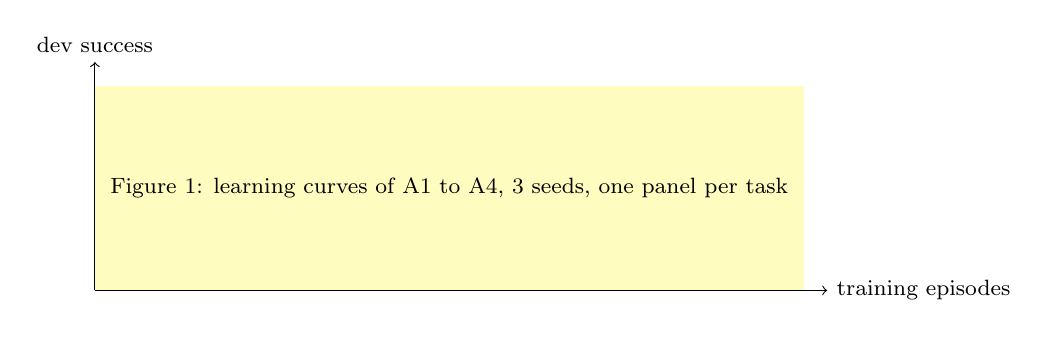
\begin{tikzpicture}[x=1cm,y=1cm]
  \fill[yellow!25] (0,0) rectangle (9,2.6);
  \draw[->] (0,0) -- (9.3,0) node[right,font=\footnotesize] {training episodes};
  \draw[->] (0,0) -- (0,2.9) node[above,font=\footnotesize] {dev success};
  \node[font=\footnotesize] at (4.5,1.3) {Figure 1: learning curves of A1 to A4, 3 seeds, one panel per task};
\end{tikzpicture}
\end{center}

\subsection*{Q4: does Gemma + Sys1 reach Qwen 27B? (the target)}

\begin{table}[H]
\scriptsize
\caption{ALFWorld test, 134 games. \emph{Best arm} is chosen on dev in Q3. Calls and tokens are per game. Agent time leaves out the game's own time. \emph{All 3 seeds} is the share of games solved by every seed, which is not $\tau$-bench's pass$^k$ over repeated trials. Gray rows ran other protocols: Bonn is picking from the list, ETO is ReAct with one example on these 134 games, and ReDAct is 400 episodes with no stated split.}
\label{t:main}
\begin{tabularx}{\linewidth}{@{}c P{6.4cm} Y Y Y Y Y Y Y Y Y Y Y Y@{}}
\toprule
Row & Who plays & Success & 95\% interval & Minus H1 & Minus H9 & Mean steps & Gemma calls & Qwen 27B calls & Sys1 share of steps & Tokens & Agent time & Repeat rate & All 3 seeds \\
\midrule
H1 & Gemma alone, picks from the list (Bonn's way) & \E & \E & n/a & \E & \E & \E & 0 & 0 & \E & \E & \E & n/a \\
H2 & Gemma alone, reasons then commands, thinking off (ReDAct's way) & \E & \E & \E & \E & \E & \E & 0 & 0 & \E & \E & \E & n/a \\
H3 & Sys1 alone, untrained & \E & \E & \E & \E & \E & 0 & 0 & 1 & 0 & \E & \E & n/a \\
H4 & Sys1 alone, best arm, 3 seeds & \E & \E & \E & \E & \E & 0 & 0 & 1 & 0 & \E & \E & \E \\
H5 & Gemma + untrained Sys1 & \E & \E & \E & \E & \E & \E & 0 & \E & \E & \E & \E & n/a \\
H6 & Gemma + Sys1, best of A1 and A2 (teacher forced only), 3 seeds & \E & \E & \E & \E & \E & \E & 0 & \E & \E & \E & \E & \E \\
H7 & Gemma + Sys1, best arm, 3 seeds (the result we want) & \E & \E & \E & \E & \E & \E & 0 & \E & \E & \E & \E & \E \\
H8 & Qwen 27B + Sys1, best arm, 3 seeds & \E & \E & \E & \E & \E & 0 & \E & \E & \E & \E & \E & \E \\
H9 & Qwen 27B alone, picks from the list (Bonn's way) & \E & \E & \E & n/a & \E & 0 & \E & 0 & \E & \E & \E & n/a \\
H10 & Qwen 27B alone, reasons then commands, thinking off (ReDAct's way) & \E & \E & \E & \E & \E & 0 & \E & 0 & \E & \E & \E & n/a \\
H11 & Gemma fine-tuned to pick the expert's command from the list, all 3,553 games, no Sys1, 3 seeds & \E & \E & \E & \E & \E & \E & 0 & 0 & \E & \E & \E & \E \\
H12 & Qwen 27B alone, thinking on at its default effort (ceiling) & \E & \E & \E & \E & \E & 0 & \E & 0 & \E & \E & \E & n/a \\
\pub & Bonn, Gemma & 6.7 & 3.0, 11.2 & & & 47.8 & & & & & & 0.541 & \\
\pub & Bonn, Qwen 27B & 54.5 & 46.3, 62.7 & & & 31.6 & & & & & & 0.272 & \\
\pub & Bonn, Jev 1.13 & 35.1 & 27.6, 43.3 & & & 37.9 & & & 1 & & & 0.447 & \\
\pub & ETO, Llama-2-7B-Chat untuned, ReAct with one example & 0.0 & & & & & & & & & & & \\
\pub & ETO, same model fine-tuned on expert games (SFT) & 67.2 & & & & & & & & & & & \\
\pub & ReDAct, Qwen3-80B alone & 68.3 & & & & & & & & & & & \\
\pub & ReDAct, GPT-5.2 alone & 78.3 & & & & & & & & & & & \\
\bottomrule
\end{tabularx}
\end{table}

\begin{table}[H]
\scriptsize
\caption{MiniGrid-DoorKey-8x8-v0 test, 200 episodes, ReDAct's seed. Same columns, with the rows that matter most.}
\label{t:mainmg}
\begin{tabularx}{\linewidth}{@{}c P{6.4cm} Y Y Y Y Y Y Y Y Y Y Y@{}}
\toprule
Row & Who plays & Success & 95\% interval & Minus H1 & Mean steps & Gemma calls & Qwen 27B calls & Sys1 share of steps & Tokens & Agent time & Repeat rate & All 3 seeds \\
\midrule
H2 & Gemma alone, reasons then commands & \E & \E & n/a & \E & \E & 0 & 0 & \E & \E & \E & n/a \\
H4 & Sys1 alone, best arm, 3 seeds & \E & \E & \E & \E & 0 & 0 & 1 & 0 & \E & \E & \E \\
H7 & Gemma + Sys1, best arm, 3 seeds (the result we want) & \E & \E & \E & \E & \E & 0 & \E & \E & \E & \E & \E \\
H8 & Qwen 27B + Sys1, best arm, 3 seeds & \E & \E & \E & \E & 0 & \E & \E & \E & \E & \E & \E \\
H10 & Qwen 27B alone, reasons then commands & \E & \E & \E & \E & 0 & \E & 0 & \E & \E & \E & n/a \\
\pub & ReDAct, Qwen3-80B alone & 85.5 & & & & & & & & & & \\
\pub & ReDAct, GPT-5.2 alone & 99.0 & & & & & & & & & & \\
\bottomrule
\end{tabularx}
\end{table}

Reading Table~\ref{t:main}: H7 against H1 and H2 asks whether Gemma gets better, and H7 against H9 and H10 asks whether it reaches Qwen 27B. H7 against H5 isolates training, H7 against H6 isolates leaving teacher forcing, H4 against H7 shows what Gemma adds to Sys1, and H11 against H7 asks whether Sys1 beats plain fine-tuning of Gemma, the usual practice in this field. Fine-tuned small models have passed 54.5 on ALFWorld in other formats (ETO 67.2 on these games, AgentGym 77.5 to 83.0 on 200 episodes, AgentTuning 84.0 on 50, each ReAct with thoughts), so Qwen 27B is the bar by your choice and not the limit of the task. H8 against H9 and H10 is your setting where the same large LLM gets shorter and more coherent runs.

\subsection*{Q5: if a few steps per game may go to Qwen 27B, how much does success rise?}

\begin{table}[H]
\footnotesize
\caption{ALFWorld test success at a fixed number of Qwen 27B calls per game, with thresholds tuned on dev. A handover here is exactly one step, so the hand-over rules are off and Sys1's row sets a threshold on its fallback probability. ReDAct tuned to 5 per episode on calibration episodes, which came to 3.6 on its test episodes. Column 0 reuses H2 and H4.}
\label{t:q5}
\begin{tabularx}{\linewidth}{@{}P{9cm} Y Y Y Y Y Y@{}}
\toprule
Who chooses the steps (columns: Qwen 27B calls per game) & 0 & 1 & 2 & 5 & 10 & Area under curve \\
\midrule
Chance: Gemma plays, random steps go to Qwen 27B & \E & \E & \E & \E & \E & \E \\
Gemma's own uncertainty: as in ReDAct, with no training & \E & \E & \E & \E & \E & \E \\
Trained Sys1: Sys1 plays, its fallback steps go to Qwen 27B & \E & \E & \E & \E & \E & \E \\
\pub ReDAct, Qwen3-80B with GPT-5.2, best uncertainty measure, 400 episodes & \multicolumn{6}{c}{80.8 at 3.6 handovers per episode} \\
\pub ReDAct, Qwen3-80B with GPT-5.2, random steps, 400 episodes & \multicolumn{6}{c}{77.0 at 3.7 handovers per episode} \\
\bottomrule
\end{tabularx}
\end{table}

\begin{center}
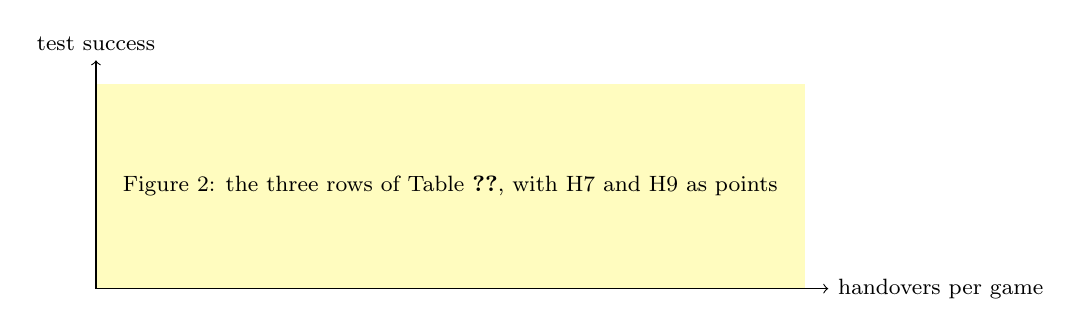
\begin{tikzpicture}[x=1cm,y=1cm]
  \fill[yellow!25] (0,0) rectangle (9,2.6);
  \draw[->] (0,0) -- (9.3,0) node[right,font=\footnotesize] {handovers per game};
  \draw[->] (0,0) -- (0,2.9) node[above,font=\footnotesize] {test success};
  \node[font=\footnotesize] at (4.5,1.3) {Figure 2: the three rows of Table~\ref{t:q5}, with H7 and H9 as points};
\end{tikzpicture}
\end{center}

\subsection*{Q6: can Sys1 stop prompt injections by checking each tool call?}

\begin{table}[H]
\footnotesize
\caption{AgentDojo workspace suite, attack \texttt{important\_instructions} (the paper's main attack), with \texttt{tool\_knowledge} as a second run, Gemma as the agent. A \emph{prompt injection} is a hidden instruction in a tool's output that tries to redirect the agent. Sys1 sees each tool call before it runs and answers pass or flag danger, and a flagged call does not run. S5 tests your claim that independence from the LLM's context helps, because an injection in a tool output cannot reach a Sys1 that never reads tool outputs. The reward comes from the suite's own security and task checks.}
\label{t:q6}
\begin{tabularx}{\linewidth}{@{}c P{8cm} Y Y Y Y Y@{}}
\toprule
Row & Defence & Task success, no attack & Task success, under attack & Attack success & False flags per 100 calls & Added seconds per call \\
\midrule
S1 & No defence & \E & \E & \E & Not applicable & 0 \\
S2 & AgentDojo \texttt{tool\_filter} & \E & \E & \E & Not applicable & \E \\
S3 & AgentDojo \texttt{PromptInjectionDetector} & \E & \E & \E & \E & \E \\
S4 & Sys1 reading the full context & \E & \E & \E & \E & \E \\
S5 & Sys1 reading only the task and the proposed call & \E & \E & \E & \E & \E \\
\pub & Ctrl-Z, BashBench, a different threat model & & & 58 to 7 & 5\% benign cost & \\
\pub & Task Shield, AgentDojo, GPT-4o, checks each call against the user's goal & \multicolumn{5}{c}{Attack success 2.07, task utility 69.79} \\
\pub & CaMeL, AgentDojo, control flow fixed from the trusted query & \multicolumn{5}{c}{77\% of tasks solved with provable security, 84\% undefended} \\
\bottomrule
\end{tabularx}

\vspace{6pt}
\begin{tabularx}{\linewidth}{@{}P{8.4cm} Y Y Y@{}}
\toprule
Optional, CyberGym 10-task subset, level 1 (counts out of 10, only with a Docker host) & Gemma alone & Gemma + Sys1 & Qwen 27B alone \\
\midrule
Tasks solved & \E & \E & \E \\
\bottomrule
\end{tabularx}
\end{table}

\subsection*{Q7: which parts of our design actually help?}

\begin{table}[H]
\scriptsize
\caption{ALFWorld test, 134 games, Gemma + Sys1, one part changed at a time, 1 seed, run after every choice is frozen, and no choice is made from this table. One seed on 134 games cannot resolve differences under about 12 points (Heuristic), so read this table as direction only. The papers we read hand one step or one move to the large model and none keeps it in control for several rounds, so the hand-over row tests what is distinctive in your design. Tier 1 is required. Tier 2 runs if time remains. R3 and R4 need Sys1 to act, so those rows run on A4.}
\label{t:abl}
\begin{tabularx}{\linewidth}{@{}P{5.7cm} P{3.2cm} P{4.2cm} c Y Y Y Y@{}}
\toprule
The part being tested & Default & Changed to & Tier & Success & Gemma calls & ECE & Repeat rate \\
\midrule
Full system & All defaults & None & 1 & \E & \E & \E & \E \\
\midrule
Control state & Seen by Sys1 & Removed & 1 & \E & \E & \E & \E \\
Menu length & $k$ tuned on dev, start 10 & $k=5$ & 1 & \E & \E & \E & \E \\
 & & $k=20$ & 1 & \E & \E & \E & \E \\
 & & All admissible commands & 1 & \E & \E & \E & \E \\
Reward & R2 & R1, your agreement reward & 1 & \E & \E & \E & \E \\
 & & R3, adds success & 1 & \E & \E & \E & \E \\
 & & R4, success only & 1 & \E & \E & \E & \E \\
Calibration step & Temperature refit & None & 1 & \E & \E & \E & \E \\
 & & Brier term in the objective & 1 & \E & \E & \E & \E \\
Teacher & Built-in expert\my & Qwen 27B games & 1 & \E & \E & \E & \E \\
Hand-over rules & 2 fallbacks, 10 rounds & None, fallback lasts one step & 1 & \E & \E & \E & \E \\
\midrule
Hand-over rules & 2 fallbacks, 10 rounds & 1 fallback, 10 rounds & 2 & \E & \E & \E & \E \\
 & & 2 fallbacks, 5 rounds & 2 & \E & \E & \E & \E \\
Trace window & Last 5 & Last 1 & 2 & \E & \E & \E & \E \\
 & & Last 20 & 2 & \E & \E & \E & \E \\
 & & Full history (Bonn) & 2 & \E & \E & \E & \E \\
LLM's last trace in Sys1's view & Seen & Removed & 2 & \E & \E & \E & \E \\
How fallback is chosen & Menu option & Threshold on confidence & 2 & \E & \E & \E & \E \\
 & & Option and threshold & 2 & \E & \E & \E & \E \\
Teacher & Built-in expert\my & Birch games, only if collected under D1 & 2 & \E & \E & \E & \E \\
Sys1 model & Kev-4B & Kev-0.8B & 2 & \E & \E & \E & \E \\
 & & decider-2b & 2 & \E & \E & \E & \E \\
 & & Clef-flash & 2 & \E & \E & \E & \E \\
Small LLM & Gemma & Qwen3.5-4B & 2 & \E & \E & \E & \E \\
\bottomrule
\end{tabularx}
\end{table}

\section{Budget and order of work}

\begin{table}[H]
\footnotesize
\caption{Runs and games. Gemma and Qwen 27B are open weights, so only a Birch teacher (D1) uses paid calls. GPU hours are filled from the first run, which goes end to end before any sweep. One 134-game pass in Bonn's way took 4,236 requests at 1.48\,s for Qwen 27B on an A100 and 6,410 at 0.27\,s for Gemma on an A40, and rows that generate text cost more. Colab: you stated about 600 hours a month. Third-party pages say Pro+ gives 500 to 600 compute units and an L4 burns 1.71 per hour, which is about 290 to 350 hours (Open: check your Colab page).}
\label{t:budget}
\begin{tabularx}{\linewidth}{@{}P{4.2cm} L P{2cm} P{2cm} c@{}}
\toprule
Experiment & Size & Training runs & Games played & GPU hours \\
\midrule
Teacher games (D1) & Expert: all 3,553 games, free. A paid LLM: 500\my{} games, at most 25,000 calls & 0 & 3,553 or 500 & \E \\
Gemma's stored picks & One forward pass at about 73,500 expert states (3,553 games, 20.7 steps), about 5.5 hours at Bonn's 0.27\,s on an A40 (Heuristic). A subset if an L4 is slower & 0 & 0 & \E \\
G & 3 players, 134 games & 0 & 402 & \E \\
Q1 & 5 LLM rows, 140 dev games & 0 & 700 & \E \\
Q2, Q3: A1, A2 & 2 arm settings, 3 seeds, 2 tasks, no live LLM & 12 & Dev only & \E \\
Q2, Q3: A3, A4 & 3 arm settings (A4 under R3 and R4), 3 seeds, 2 tasks, Gemma live & 18 & Dev only & \E \\
Q4 ALFWorld & 12 rows, 20 runs with seeds, 134 games. H1 and H9 reuse G & 3 & 2,680 & \E \\
Q4 MiniGrid & 5 rows, 11 runs with seeds, 200 episodes & 0 & 2,200 & \E \\
Q5 & 3 rows, 1, 2, 5 and 10 handovers, 134 games & 0 & 1,608 & \E \\
Q6 & 5 rows, S4 and S5 at 3 seeds, workspace cases & 6 & Case counts & \E \\
Q7 & 11 changes in Tier 1 and 13 in Tier 2, 134 games each. The small-LLM row and the threshold rows need no retraining & 21 & 3,216 & \E \\
\bottomrule
\end{tabularx}
\end{table}

The order follows the story: G, Q1, one run end to end, Q2 and Q3 on ALFWorld, Q4 on ALFWorld, then Q5, Q6, MiniGrid and Q7. The syllabus and guidelines give no dates for the later milestones, so this mapping is by content\my. The Formulation and Design Report carries the harness, the arms and G. The Progress and Evaluation Report carries Q1 to Q4 on ALFWorld. The presentation and final report carry the rest.

The cut order when time runs short\my{} is ScienceWorld, CyberGym, MiniGrid, Tier 2, Q6, A3. G, Q1, the arms A1, A2 and A4, and Q4 on ALFWorld survive every cut. The last resort is your reduced project: a System One tool selector on BFCL v4 with A0, A1 and A2, which still measures the effect of RL training.

\section*{Appendix: changes from the proposal}

The proposal says the formulation can change, and the Formulation and Design Report is where the change gets stated. Tasks move from $\tau$-bench to ALFWorld and MiniGrid, so the simulated user leaves the environment. A menu of frequent tool calls becomes frequent kinds of command filled in from the admissible commands, which settles the open question on arguments. The small LLM is now Gemma and the strong second setting is Qwen 27B. CyberGym moves to optional and AgentDojo carries security, as you suggested with ``another task for guardrail part''. Sys1's action set, the hand-over rules, the fallback label, teacher forcing as a research path, the control state and the comparison with the LLM alone are unchanged. ALFWorld commands are not tool calls, so Q6 is the only literal tool-calling evidence in the core plan (Open whether Q4 transfers to it). The course requires an LLM-use disclosure with each deliverable, and this plan should appear in the next one.

\section*{Appendix: comparison papers}

\begin{table}[H]
\footnotesize
\caption{Why these two models: who else uses them. Only Bonn uses both on one task, and only Bonn uses either on ALFWorld. When2Ask, SwiftSage and ReDAct use neither. We found no work that trains a Sys1 to lift Gemma. This comes from web searches, so a missed paper is possible. Bellman Language Models and MobilePA-Bench also use Qwen 27B and are in the next table. All numbers are Empirical on the setup stated.}
\label{t:prior}
\begin{tabularx}{\linewidth}{@{}P{5.2cm} P{1.9cm} P{5.2cm} L@{}}
\toprule
Work & Uses & Task, and how the model runs & Published number \\
\midrule
Bonn, arXiv 2609.37647 & Both & ALFWorld and 37 datasets, as reference models beside Jev. Thinking off, one forward pass & ALFWorld success: Gemma 6.7, Qwen 27B 54.5 \\
Gemma model card & Gemma & $\tau^2$, settings not given & 42.2\% average over 3 \\
Small coding agents, arXiv 2610.33958 & Gemma & SWE-bench Verified issue localization, tool ablation, models from 0.6B to 32B & Function Acc@10 on 500 tasks: 16.7 with grep tools, 29.7 with all tools \\
Not Every Call Needs a Frontier Model, arXiv 2610.09021 & Gemma & Five call sites of a home-automation agent, one of seven local models, 4-bit & Overall 78.6, best local model for one call site \\
Dense and MoE study, arXiv 2604.07035 & Gemma & ARC, GSM8K, Math, TruthfulQA. No agent & Mean VRAM 14.9\,GB \\
Clef, Kev, JEV-27B & Qwen 27B & Open Sys1 models built on it or offered on it. Your Cloudflare idea starts here & Clef card numbers in the appendix \\
\bottomrule
\end{tabularx}
\end{table}

\begin{table}[H]
\scriptsize
\caption{All numbers are Empirical, on the setup stated, and none predicts ours. The last column is what we copy so our rows read beside theirs.}
\label{t:comp}
\begin{tabularx}{\linewidth}{@{}P{2.3cm} P{4.1cm} P{4.3cm} L P{4.6cm}@{}}
\toprule
Work & Tasks & Method and models & Published result & What we copy \\
\midrule
Bonn/Lamarr, arXiv 2609.37647 & ALFWorld unseen, 134 games, 50 steps. Also TextWorld, BabyAI-Text, FrozenLake & Untrained pick over admissible commands. Jev 1.13, Qwen 27B, Gemma. MIT code and raw data & Success: Jev 35.1 [27.6, 43.3], Qwen 27B 54.5 [46.3, 62.7], Gemma 6.7 [3.0, 11.2], built-in expert 90.3 & Games, state, success, repeat rate, step agreement, ECE, Brier, and G \\
ReDAct, arXiv 2604.07036 & ALFWorld 400 episodes, 50 steps. MiniGrid DoorKey-8x8, 200 episodes & Threshold on action-level uncertainty, no training, tuned to about 5 large calls per episode. Small Qwen3-80B and others, large GPT-5.2 and others. No code link & ALFWorld: Qwen3-80B 68.3, GPT-5.2 78.3 with 9,898 large calls, best handover 80.8 with 1,447, random handover 77.0 with 1,487. MiniGrid: Qwen3-80B 85.5, with handover 93.0 to 95.0, random handover 93.0, GPT-5.2 99.0 & Reasoning then a command, the uncertainty and random rows of Q5, MiniGrid seeds, cost columns. Its plus-minus values are bootstrap standard deviations, and its 400 ALFWorld episodes have no stated split \\
ETO, arXiv 2403.02502 & ALFWorld 134 unseen games, also WebShop and ScienceWorld & Llama-2-7B-Chat fine-tuned on 3,321 expert instances, then contrastive exploration. ReAct with one example & Untuned 0.0, SFT 67.2, PPO 29.1, ETO 72.4, GPT-4 38.1 & The fine-tuning row H11, and evidence that imitation is the usual start \\
AgentTuning, arXiv 2310.12823 & AgentBench's ALFWorld, 50 instances & Llama-2 fine-tuned on 336 success-filtered GPT-4 ReAct trajectories out of 954 & 7B chat 2.0, AgentLM-7B 84.0, GPT-4 78.0 & Filtering teacher games by success (our C8) \\
AgentGym, arXiv 2406.04151 & ALFWorld, 200 evaluation instructions & Behaviour cloning on 2,420 trajectories, then agent evolution & Llama-2-7B 2.0, BC 77.5 and 83.0, GPT-4-Turbo 67.5 & Same \\
BUTLER, ALFWorld paper, arXiv 2010.03768 & ALFWorld, 50K episodes & DAgger with the handcoded expert, whose share falls from 100\% to 1\%, 8 seeds, text generation & Read at setup & The schedule idea in A3 \\
TWOSOME, arXiv 2401.14151 & VirtualHome and Overcooked, up to 500k steps & PPO with LoRA on frozen LLaMA-7B, scoring all valid actions by likelihood, 3 seeds & Reports better sample efficiency than plain PPO and SayCan & The closest method to A4 \\
GLAM, arXiv 2302.02662 & BabyAI-Text, 1.5M steps, 6 actions & PPO on Flan-T5 780M scoring valid actions, 4 seeds & Read at setup & RL budgets on action lists \\
Bellman Language Models, arXiv 2610.24871 & $\tau^2$ telecom, SymPy issues, Mozilla CI triage, InventoryBench & Controller built from a solved decision process over discretized conversation states, from logs or the agent's own runs. Moves fixed by the state are sent directly, and unseen states go back to the LLM. The abstract names no RL. Preregistered, no code link & Telecom, tasks solved of 114, Qwen 27B alone then with BLM: 52 to 94, 31 to 102, 33 to 109. Same set as 31 to 102, Qwen 27B alone with thinking 62. SymPy 14 to 19 of 63, not significant & Closest recent work on a controller around an LLM. No Gemma, no ALFWorld \\
MobilePA-Bench, arXiv 2608.23035 & Mobile planning sandbox & Qwen 27B trained with online GRPO, 4,000 queries, one exploratory checkpoint & Overall score 66.94 to 69.25 & Precedent for RL on Qwen 27B itself \\
When2Ask, arXiv 2306.03604 & MiniGrid variants, Habitat & PPO policy on when to ask, penalty when the plan does not change. Vicuna-7b, 13b. Baselines Hard-coded, Always, Random, Never & Reports LLM interaction counts & RL on when to call the LLM \\
SwiftSage, arXiv 2305.17390 & ScienceWorld, 30 task types & T5-large by behaviour cloning, generative, with GPT-4 and a heuristic switch & Average score 84.7 & Extension task and its score \\
RelayLLM, arXiv 2601.05167 & Math benchmarks & Qwen3-0.6B, 1.7B call Qwen3-8B. Supervised warm-up, then GRPO, reward is correctness minus call ratio & Qwen3-1.7B 42.50 to 49.52 with 1.07\% of tokens, teacher alone 54.12 & Reporting token share beside accuracy \\
\bottomrule
\end{tabularx}
\end{table}

\begin{table}[H]
\scriptsize
\caption{Comparison papers, continued: System One vendors and security. Same reading as the table before.}
\begin{tabularx}{\linewidth}{@{}P{2.3cm} P{4.1cm} P{4.3cm} L P{4.6cm}@{}}
\toprule
Work & Tasks & Method and models & Published result & What we copy \\
\midrule
decider v8 to v10 & 16 live MiniWoB++ click tasks and games & PPO on the served softmax for 384 steps after supervised training, with a KL term to the supervised weights. Recipe in \texttt{docs/RL.md}, training code kept separate & Vendor report & PPO on a softmax over options \\
Clef card, CLM post & BFCL, ToolRet, BANKING77. BFCL v4, T-Rex, WikiRacing, Mario & Schema head, or state-action scorer on Qwen3-8B. Supervised, as Kev's card also describes, with a fitted temperature. Self-reported & Clef: BFCL 98.5, ToolRet 69.2. CLM: ``on par'' with Jev & Tasks for the reduced project \\
AgentDojo, arXiv 2406.13352 & 97 user tasks, 629 security cases & \texttt{tool\_filter}, \texttt{PromptInjectionDetector}, main attack \texttt{important\_instructions} & Read from its results at setup & The suite, the checker, the defence rows \\
Ctrl-Z, arXiv 2504.10374 & BashBench, 257 tasks & Control protocols that resample suspicious commands & Attack success 58\% to 7\% at 5\% benign cost & Reporting attack success beside benign cost \\
CyberGym, ICLR 2026 & 1,507 tasks & Measures exploitation capability & Read at setup if run & Counts on its 10-task subset \\
\bottomrule
\end{tabularx}
\end{table}

\end{document}
